\documentclass{article}
\usepackage{ctex}
\usepackage[margin=1in]{geometry}
\usepackage{lineno,hyperref, tablefootnote, booktabs, graphicx, subfigure, amsmath, multirow}
\title{机器学习概论\\实验一~垃圾邮件识别}
\author{张晨~2017011307}
\date{}

\begin{document}

\maketitle

\section{基本原理}
已知训练集集中标签$y$(是垃圾邮件/不是垃圾邮件)的出现概率$P(y)$,每种标签下各个词项$x_i$的出现概率$P\left(x_{i} | y\right)$,可根据下式估算测试集中一个拥有词项$x_1, ... ,x_n$的邮件的标签为$y$的概率。
\begin{equation}
\label{equ:bayes}
P\left(y | x_{1}, \ldots, x_{n}\right) =  P(y) \prod_{i=1}^{n} P\left(x_{i} | y\right)
\end{equation}
测试集中,邮件的标签输出为概率最大的标签,即
\begin{equation}
\hat{y}=argmax_{y} P(y) \prod_{i=1}^{n} P\left(x_{i} | y\right)
\end{equation}
为了保证运算精度,在实际计算过程中,会对等式两边同时取对数。
\section{对正文的处理}
\subsection{预处理}
\paragraph{数据集选取} 数据集中共37822封邮件,其中 python 可直接读取的有32401封。为分析便利,取其中32400封。
将这些邮件打乱顺序后,分为5折。
\paragraph{元数据与正文的分离} 观察发现,在绝大多数的文章中,元数据与正文以一个空行分割。
个别的例外,如118/184等,暂不考虑。
\paragraph{异常邮件的处理} 共有528封完全为base64编码的邮件,其中垃圾邮件505封,非垃圾邮件23封。
在测试时,将它们都归为垃圾邮件。此外,有142封邮件中出现了形如``B--------"的串,
它们的内容均为乱码,分类全是垃圾邮件,故在测试时,直接标记为垃圾邮件。

\subsection{基础版本的实现}
训练阶段,将训练集中邮件的正文进行分词,统计各个词项出现的次数,留下出现次数大于等于10的词项。分词的限制较松,允许一些非单词的元素出现,但会将单词最后的句号去掉。

测试阶段,对于测试集中的每封邮件,用同样的方法进行分词。若某个词项仅在垃圾邮件中出现过,则标记为垃圾邮件,若某个词项仅在非垃圾邮件中出现过,标记为非垃圾邮件。否则使用公式\ref{equ:bayes}进行计算。

此版本的准确率如下表所示。
\begin{table}[h]
\center
\label{tab:naive}
\begin{tabular}[]{|c|c|c|c|}
\hline
Accuracy & Precision & Recall & F1 \\ \hline
 0.9724 & 0.9945 & 0.9607 & 0.9773 \\ \hline
\end{tabular}
\end{table}
\subsection{使用词表}
在基础版本中,词项中有很多非单词的元素。我使用一个20000个单词的词表进行过滤,仅保留词表中的单词。
同时,我还测试了词表中单词+垃圾邮件中的词项,词表中单词+非垃圾邮件中的词项两种组合,以及忽略大小写的结果。
实验结果如下。
\begin{table}[h]
\center
\label{tab:wordlist}
\begin{tabular}[]{|c|c|c|c|c|}
\hline
& Accuracy & Precision & Recall & F1 \\ \hline
仅含词表中单词 & 0.9404 & 0.9955 & 0.9079 & 0.9496 \\ \hline
词表单词+垃圾邮件词项 & 0.9718 & 0.9923 & 0.9619 & 0.9769 \\ \hline
词表单词+非垃圾邮件词项 & 0.9467 & 0.9962 & 0.9174 & 0.9552 \\ \hline
仅含词表中单词,忽略大小写 & 0.8833 & 0.9949 & 0.8157 & 0.8962 \\ \hline
\end{tabular}
\end{table}
\subsection{停用词}
一般而言,在进行文本分析的时候,需要删除停用词。我也对此作了测试,实验结果如下。可见,删除停用词会略微提高准确度。
\begin{table}[h]
\center
\label{tab:stopwords}
\begin{tabular}[]{|c|c|c|c|c|}
\hline
& Accuracy & Precision & Recall & F1 \\ \hline
全体词项删除停用词 & 0.9733 & 0.9941 & 0.9626 & 0.9781 \\ \hline
词表单词删除停用词 & 0.9505 & 0.9949 & 0.9247 & 0.9585 \\ \hline
\end{tabular}
\end{table}
\newpage
\subsection{截取长度}
出现次数较少的词项,在两种标签中的出现概率随机性较大,故可靠性可能降低。但是,实验发现,在这个数据集中,不删除任何词项却是准确度最高的做法。这是邮件的内容重复造成的,在后面会具体分析。之后的实验,都不再进行频率的截取。具体数据如下
\begin{figure}[h]
    \centering
    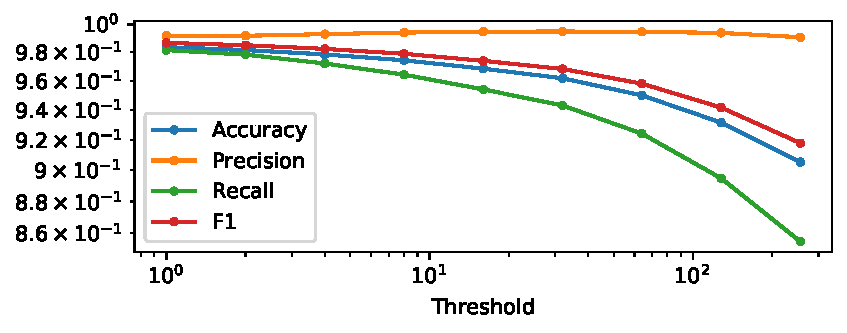
\includegraphics{figure/trunc.pdf}
    \label{fig:trunc}
\end{figure}

\subsection{提升precision或recall}
若想提高precision,可提高垃圾邮件的判别条件,若想提高recall,可降低垃圾邮件的判别条件。我分别尝试了这两种做法,与预想一致,结果如下
\begin{table}[h]
\center
\label{tab:rate}
\begin{tabular}[]{|c|c|c|c|c|}
\hline
&Accuracy & Precision & Recall & F1 \\ \hline

    提高一倍非垃圾邮件词频 & 0.9873 & 0.9935 & 0.9859 & 0.9897 \\ \hline
    正常&0.9887 & 0.9970 & 0.9848 & 0.9908 \\ \hline
    提高一倍垃圾邮件词频 & 0.9887 & 0.9972 & 0.9844 & 0.9908 \\ \hline

\end{tabular}
\end{table}

\section{零概率的处理}
\subsection{平滑}
对于仅在垃圾邮件中出现或仅在非垃圾邮件中出现的词项,直接进行计算会由于计算$log(0)$而出错。通用的解决方法是进行平滑。平滑参数$\alpha$的选取与准确度的关系如下表所示。
\begin{table}[h]
\center
\label{tab:zero}
\begin{tabular}[]{|c|c|c|c|c|}
\hline
$\alpha$ & Accuracy & Precision & Recall & F1 \\ \hline
0.01 & 0.9642 & 0.9967 & 0.9451 & 0.9702 \\ \hline
0.1 & 0.9565 & 0.9959 & 0.9334 & 0.9636 \\ \hline
0.5 & 0.9452 & 0.9955 & 0.9154 & 0.9538 \\ \hline
1 & 0.9372 & 0.9951 & 0.9029 & 0.9467 \\ \hline
2 & 0.9290 & 0.9943 & 0.8904 & 0.9394 \\ \hline
\end{tabular}
\end{table}
从表中可以看出,无论平滑参数如何选取,准确率都低于直接判断(若某个词项仅在垃圾邮件中出现过,则标记为垃圾邮件,若某个词项仅在非垃圾邮件中出现过,标记为非垃圾邮件)
\subsection{直接判断}
进一步分析发现,绝大部分的邮件,都可以使用直接判断的方法进行处理,且准确率较高,具体如下表所示
\begin{table}[h]
\center
\label{tab:split}
\begin{tabular}[]{|c|c|c|c|c|c|}
\hline
& 总数 &Accuracy & Precision & Recall & F1 \\ \hline
异常邮件 (判为垃圾邮件)& 670 & 0.9658 & 0.9658 & 1.0000 & 0.9826 \\ \hline
仅含在垃圾邮件中出现过的零概率词项 & \multirow{2}*{18499} & \multirow{2}*{0.9993} & \multirow{2}*{0.9993} & \multirow{2}*{1.0000} & \multirow{2}*{0.9996} \\ 
(判为垃圾邮件) & ~ & ~ & ~ & ~ & ~ \\ \hline
仅含在非垃圾邮件中出现过的零概率词项 & \multirow{2}*{10416} &\multirow{2}*{0.9954} & \multirow{2}*{0.0000} & \multirow{2}*{0.0000} & \multirow{2}*{0.0000} \\
(判为非垃圾邮件) & ~ & ~ & ~ & ~ & ~ \\ \hline
两种零概率词项都有(根据出现频次之和判断)& 2419 & 0.9112 & 0.9704 & 0.7403 & 0.8393 \\ \hline
无零概率词项 & 396 & 0.8297 & 0.8256 & 0.3175 & 0.4377 \\ \hline
\end{tabular}
\end{table}

从上表可以看出,若仅含在一种标签中的零概率词项,直接将其判为该标签可获得极高的准确率。一个可能的原因是,数据集较小,且存在重复(如001/176和001/200除时间外完全一样)。
\textbf{为更明显的反映不同方法的意义,在之后的实验中,如没有特别说明,则忽略这些测例。}忽略这些测例后,剩余测例的accuracy仅为0.86。


\section{元数据的使用}
\subsection{标题}
\subsubsection{词频法}
标题与正文结合有两种办法,一是为标题赋予较大的权重,与正文合并为同一词表。二是为标题和正文分别构建词表。在我的实验中,方法二效果较好。比较有意思的一点是,在这些测例中,仅考虑标题的准确度要高于仅考虑文本,其原因可能是,文本中存在大量非文字内容,会影响判断。
\begin{table}[h]
\center
\label{tab:meta-title}
\begin{tabular}[]{|c|c|c|c|c|}
\hline
& Accuracy & Precision & Recall & F1 \\ \hline
仅使用标题 & 0.8893 & 0.8701 & 0.7432 & 0.8012 \\ \hline
仅使用文本 & 0.8697 & 0.9684 & 0.5876 & 0.7283 \\ \hline
单词表,标题权重1 & 0.8761 & 0.9585 & 0.6162 & 0.7475 \\ \hline
单词表,标题权重10 & 0.8899 & 0.9649 & 0.6602 & 0.7809 \\ \hline
单词表,标题权重100 & 0.9176 & 0.9479 & 0.7686 & 0.8483 \\ \hline
双词表,标题权重1 & 0.8816 & 0.9577 & 0.6364 & 0.7619 \\ \hline
双词表,标题权重10 & 0.8999 & 0.9595 & 0.6980 & 0.8065 \\ \hline
双词表,标题权重100 & 0.9200 & 0.9378 & 0.7856 & 0.8541 \\ \hline
\end{tabular}
\end{table}

\subsubsection{其他特征}
我猜想在回复的邮件中,垃圾邮件极少,但对整个数据集统计发现,带有标题中带有``Re:"的邮件中,垃圾/非垃圾的比例为2662/5119,差距不悬殊。再加上在词频分析中,已经间接考虑了``Re"一词,我就不再对其进行特殊处理。

我的另外一个猜想是,标题中带有感叹号的,垃圾邮件较多。但实际统计发现,在整个数据集上,差距并不显著,且带有感叹号的标题仅占所有标题的一小部分,故我认为该特征不会带来明显的效果提升,也未做进一步测试。

\subsection{客户端}
垃圾邮件的分布与客户端有一定的关联性,如``devMail.Net"发出的1537封邮件,全是垃圾邮件,``Mozilla"发出的1259封邮件,仅有2封不是垃圾邮件。但加入这个特征之后,模型的表现基本不变。具体数据如下。本着模型应尽量简单的原则,我放弃了这个特征。
\begin{table}[h]
\center
\label{tab:meta-mailer}
\begin{tabular}[]{|c|c|c|c|c|}
\hline
客户端权重&Accuracy & Precision & Recall & F1 \\ \hline
1& 0.9200 & 0.9378 & 0.7856 & 0.8541 \\ \hline
2& 0.9204 & 0.9379 & 0.7869 & 0.8550 \\ \hline
4& 0.9201 & 0.9394 & 0.7848 & 0.8542 \\ \hline
8& 0.9205 & 0.9355 & 0.7898 & 0.8557 \\ \hline

\end{tabular}
\end{table}

\subsection{发送方}
在我解析出的发送方中,全为垃圾邮件的有5320个地址,全为非垃圾邮件的有1150个地址,垃圾邮件、非垃圾邮件都有的仅有11个地址。我将在训练集中全是垃圾邮件的发送方标记为黑名单,所有邮件全判为垃圾邮件;训练集中全是非垃圾邮件的发送方标记为白名单,所有邮件全判为非垃圾邮件。因为两种邮件都有的地址很少,我没有将其作为模型的一个特征。然而,加入黑白名单,并没有明显提升模型的表现,具体数据如下。
\begin{table}[h]
\center
\label{tab:meta-sender}
\begin{tabular}[]{|c|c|c|c|}
\hline
Accuracy & Precision & Recall & F1 \\ \hline
0.9207 & 0.9401 & 0.7856 & 0.8551 \\ \hline
\end{tabular}
\end{table}

\section{训练集大小}
最后,我测试了训练集规模对结果的影响,测试方法是在五折交叉验证的基础上,对训练集进行不同比例的采样,每个比例重复多次,并在整个测试集上进行测试。模型表现统计如下。可以发现,在目前的规模下,增大训练集规模可以明显的减小错误率。其根源可能为3.2节所述的直接判断法。
\newpage
\begin{table}[h]
\center
\label{tab:size}
\begin{tabular}[]{|c|c|c|c|c|c|c|c|c|c|c|c|c|c|c|c|c|}
\hline
\multirow{2}*{截取比例}& \multicolumn{3}{|c|}{Accuracy} & \multicolumn{3}{|c|}{Precision} & \multicolumn{3}{|c|}{Recall} & \multicolumn{3}{|c|}{F1} \\ \cline{2-13}
~& max & min & avg & max & min & avg & max & min & avg & max & min & avg \\ \hline
0.05 & 0.955&0.950&0.953&0.983&0.979&0.980&0.949&0.939&0.943&0.963&0.959&0.961 \\ \hline
0.5 & 0.985&0.984&0.984&0.995&0.994&0.995&0.981&0.979&0.980&0.988&0.987&0.987 \\ \hline
1 & 0.991&0.991&0.991&0.996&0.996&0.996&0.989&0.989&0.989&0.992&0.992&0.992 \\ \hline
\end{tabular}
\end{table}
\section{最终结果}
最终模型采用了如下方法
\begin{itemize}
    \item 异常邮件,直接标注为垃圾邮件
    \item 去除停用词
    \item 若所有零概率词项都出自垃圾邮件,则判为垃圾邮件;若所有零概率词项都出自非垃圾邮件,则判为非垃圾邮件。
    \item 剩余邮件的零概率词项进行平滑
    \item 若发件人位于黑名单中,判为垃圾邮件;若发件人位于白名单中,判为非垃圾邮件。
    \item 使用朴素贝叶斯公式分别处理标题和正文,并以一定权重结合。
\end{itemize}

在整个数据集上采用五折交叉验证的准确率如下
\begin{table}[h]
\center
\label{tab:final}
\begin{tabular}[]{|c|c|c|c|}
\hline
Accuracy & Precision & Recall & F1 \\ \hline

    0.9918 & 0.9959 & 0.9908 & 0.9933 \\ \hline

\end{tabular}
\end{table}

\section{总结}
这次实验,我感受了常见文本处理思路在文本分类上的作用,并进一步熟悉了贝叶斯算法。直接判断法的效果着实令我惊讶,但这并不是一个通用的方法,若数据集增大,它会失效。
\end{document}

